% Options for packages loaded elsewhere
\PassOptionsToPackage{unicode}{hyperref}
\PassOptionsToPackage{hyphens}{url}
%
\documentclass[
  12pt,
]{article}
\usepackage{amsmath,amssymb}
\usepackage{lmodern}
\usepackage{iftex}
\ifPDFTeX
  \usepackage[T1]{fontenc}
  \usepackage[utf8]{inputenc}
  \usepackage{textcomp} % provide euro and other symbols
\else % if luatex or xetex
  \usepackage{unicode-math}
  \defaultfontfeatures{Scale=MatchLowercase}
  \defaultfontfeatures[\rmfamily]{Ligatures=TeX,Scale=1}
\fi
% Use upquote if available, for straight quotes in verbatim environments
\IfFileExists{upquote.sty}{\usepackage{upquote}}{}
\IfFileExists{microtype.sty}{% use microtype if available
  \usepackage[]{microtype}
  \UseMicrotypeSet[protrusion]{basicmath} % disable protrusion for tt fonts
}{}
\makeatletter
\@ifundefined{KOMAClassName}{% if non-KOMA class
  \IfFileExists{parskip.sty}{%
    \usepackage{parskip}
  }{% else
    \setlength{\parindent}{0pt}
    \setlength{\parskip}{6pt plus 2pt minus 1pt}}
}{% if KOMA class
  \KOMAoptions{parskip=half}}
\makeatother
\usepackage{xcolor}
\usepackage[margin=1in]{geometry}
\usepackage{longtable,booktabs,array}
\usepackage{calc} % for calculating minipage widths
% Correct order of tables after \paragraph or \subparagraph
\usepackage{etoolbox}
\makeatletter
\patchcmd\longtable{\par}{\if@noskipsec\mbox{}\fi\par}{}{}
\makeatother
% Allow footnotes in longtable head/foot
\IfFileExists{footnotehyper.sty}{\usepackage{footnotehyper}}{\usepackage{footnote}}
\makesavenoteenv{longtable}
\usepackage{graphicx}
\makeatletter
\def\maxwidth{\ifdim\Gin@nat@width>\linewidth\linewidth\else\Gin@nat@width\fi}
\def\maxheight{\ifdim\Gin@nat@height>\textheight\textheight\else\Gin@nat@height\fi}
\makeatother
% Scale images if necessary, so that they will not overflow the page
% margins by default, and it is still possible to overwrite the defaults
% using explicit options in \includegraphics[width, height, ...]{}
\setkeys{Gin}{width=\maxwidth,height=\maxheight,keepaspectratio}
% Set default figure placement to htbp
\makeatletter
\def\fps@figure{htbp}
\makeatother
\setlength{\emergencystretch}{3em} % prevent overfull lines
\providecommand{\tightlist}{%
  \setlength{\itemsep}{0pt}\setlength{\parskip}{0pt}}
\setcounter{secnumdepth}{5}
\newlength{\cslhangindent}
\setlength{\cslhangindent}{1.5em}
\newlength{\csllabelwidth}
\setlength{\csllabelwidth}{3em}
\newlength{\cslentryspacingunit} % times entry-spacing
\setlength{\cslentryspacingunit}{\parskip}
\newenvironment{CSLReferences}[2] % #1 hanging-ident, #2 entry spacing
 {% don't indent paragraphs
  \setlength{\parindent}{0pt}
  % turn on hanging indent if param 1 is 1
  \ifodd #1
  \let\oldpar\par
  \def\par{\hangindent=\cslhangindent\oldpar}
  \fi
  % set entry spacing
  \setlength{\parskip}{#2\cslentryspacingunit}
 }%
 {}
\usepackage{calc}
\newcommand{\CSLBlock}[1]{#1\hfill\break}
\newcommand{\CSLLeftMargin}[1]{\parbox[t]{\csllabelwidth}{#1}}
\newcommand{\CSLRightInline}[1]{\parbox[t]{\linewidth - \csllabelwidth}{#1}\break}
\newcommand{\CSLIndent}[1]{\hspace{\cslhangindent}#1}
\usepackage{rotating}
\usepackage{setspace}
\usepackage{lineno}
\usepackage{booktabs}
\usepackage{longtable}
\usepackage{array}
\usepackage{multirow}
\usepackage{wrapfig}
\usepackage{float}
\usepackage{colortbl}
\usepackage{pdflscape}
\usepackage{tabu}
\usepackage{threeparttable}
\usepackage{threeparttablex}
\usepackage[normalem]{ulem}
\usepackage{makecell}
\usepackage{xcolor}
\ifLuaTeX
  \usepackage{selnolig}  % disable illegal ligatures
\fi
\IfFileExists{bookmark.sty}{\usepackage{bookmark}}{\usepackage{hyperref}}
\IfFileExists{xurl.sty}{\usepackage{xurl}}{} % add URL line breaks if available
\urlstyle{same} % disable monospaced font for URLs
\hypersetup{
  pdftitle={Grief and Anger: Disentangling the Effects of COVID-19 on Turnout},
  pdfauthor={Kevin Morris},
  hidelinks,
  pdfcreator={LaTeX via pandoc}}

\title{Grief and Anger: Disentangling the Effects of COVID-19 on Turnout\thanks{Thanks.}}
\author{Kevin Morris\footnote{Researcher, Brennan Center for Justice at NYU School of Law, 120 Broadway Ste 1750, New York, NY 10271 (\href{mailto:kevin.morris@nyu.edu}{\nolinkurl{kevin.morris@nyu.edu}})}}
\date{January 19, 2023}

\begin{document}
\maketitle
\begin{abstract}
The novel coronavirus SARS-CoV-2 (COVID-19) upended normal routines across the United States. Nearly 600 thousand Americans have died of COVID-19, and more than 33 million have tested positive for the illness. At the same time, there is widespread perception that the government's response to the pandemic has been lackluster, and the racial disparities are clear. This manuscript tests whether COVID mobilized nonwhite voters to participate on the basis of political threat, or was simply a discouraging event. By leveraging individual-level death records from Washington State, I identify registered voters who lived with individuals who died from COVID- 19, testing whether this was a mobilizing effect, especially for non-white voters. These analyses are supplemented with survey data exploring whether COVID-19 was differ- ently mobilizing for voters depending on how close they feel to their racial or ethnic group.
\end{abstract}

\pagenumbering{gobble}
\pagebreak

\pagenumbering{arabic}
\doublespacing

\hypertarget{introduction}{%
\subsection*{Introduction}\label{introduction}}
\addcontentsline{toc}{subsection}{Introduction}

Introduction
On January 21, 2020, the first case of SARS-CoV-2 (or ``COVID-19'') was confirmed in the state of Washington (\protect\hyperlink{ref-McNerthney2020}{McNerthney 2020}). President Donald Trump made his first public comments on the new virus the next day from Davos, telling CNBC ``we have it totally under control. It's one person coming in from China, and we have it under control'' (\protect\hyperlink{ref-Calia2020}{Calia 2020}). A few days later, on January 30, he said at a manufacturing plant in Michigan that ``we think we have it very well under control,'' assuring listeners that ``it's going to have a very good ending for it'' (\protect\hyperlink{ref-whitehouse2020}{{``Remarks by {President Trump} at a {USMCA Celebration} with {American Workers}''} 2020}). Meanwhile, cases were identified in states across the country. The first confirmed death attributed to COVID-19 occurred in Northern California on February 4th (\protect\hyperlink{ref-Moon2020}{Moon 2020}). By early March, Washington State was being called the center of the outbreak in the United States (\protect\hyperlink{ref-Golden2020}{Golden 2020}), although New York City would soon claim that dubious honor. By the time of the 2020 presidential election, more than 8.3 million Americans had tested positive for the novel coronavirus, with more than 220 thousand dead (\protect\hyperlink{ref-nyt2020}{{``Covid in the {U}.{S}.: {Latest Map} and {Case Count}''} 2020}). Reporting from a few months earlier, however, indicates that the official reports may be undercounts (\protect\hyperlink{ref-Lu2020}{Lu 2020}).

Although the World Health Organization declared COVID-19 a pandemic on March 11 (\protect\hyperlink{ref-Wan2020}{Wan 2020}), the response from the United States' federal government was slow. In the months to come, the Trump Administration would push responsibility to states and local governments, downplay the severity of the pandemic, and argue against the widespread stay-at-home orders promoted by public health experts (\protect\hyperlink{ref-Shear2020}{Shear et al. 2020}). Much of the United States remained at home throughout the summer even as peer nations were able to return to more normal daily life (\protect\hyperlink{ref-Douglas2020}{Douglas 2020}). The Trump Administration's response to the pandemic was consistently criticized in the press, with Time Magazine arguing that a ``complete catalog of Trump's failures to adequately address the pandemic is the stuff of books, not single articles'' (\protect\hyperlink{ref-Fitzpatrick2020}{Fitzpatrick 2020}).

The COVID-19 pandemic did not hit all Americans equally. A burgeoning literature is beginning to examine the racially disparate impact the virus has had on communities of color---and, in particular, Black communities. Although comprehensive data are not available in all states, an early study looked at the racial breakdown in hospitalizations in 12 states between April 30 and June 24, 2020 (\protect\hyperlink{ref-Karaca-Mandic2021}{Karaca-Mandic, Georgiou, and Sen 2021}). In each of the 12 states, whites made up a far lower share of the hospitalized population than the statewide residential population, while ``the percentage of hospitalizations among Black patients exceeded the percentage of their representative proportion of the state population in all 12 states'' (\protect\hyperlink{ref-Karaca-Mandic2021}{Karaca-Mandic, Georgiou, and Sen 2021, 133}). Similarly, a report from the Centers for Disease Control and Prevention found evidence of highly racially disparate hospitalization rates early in the pandemic (\protect\hyperlink{ref-Garg2020}{Garg et al. 2020}). These trends continued into the spring of 2021---as of April 23rd that year, Black and Latino Americans had died from COVID-19 at roughly twice the rate of white Americans; this figure was even higher for Native Americans (\protect\hyperlink{ref-cdc2021}{{``Cases, {Data}, and {Surveillance}''} 2021}). Scholars are already identifying the ways in which systemic racism---and not ``inherent'' or ``biological'' racial differences---have led to these discrepancies (\protect\hyperlink{ref-Johnson-Agbakwu2020}{Johnson-Agbakwu et al. 2020}; \protect\hyperlink{ref-Egede2020}{Egede and Walker 2020}).

Our understanding of the electoral effects of threatening policy has grown in recent years, with scholars arguing that discriminatory governmental (in)action can lead to higher voter turnout among impacted communities (\protect\hyperlink{ref-HoSang2010}{HoSang 2010}). The COVID-19 pandemic presents a unique opportunity to extend our understanding of the mechanisms of this ``political threat,'' particularly as it applies to racial and ethnic minorities. When citizens feel that they are being targeted by their government because of their racial or ethnic identity, such targeting can lead to greater political knowledge, higher likelihood of attending protests, and increased propensity to cast a ballot. Sometimes framed as backlash against a racially discriminatory government, it seems that---under certain circumstances---racial minorities understand the political sphere as a site for contesting this aggressive state action.

At the same time, many of these ``political threats'' that have spurred increased turnout among minorities are also linked with \emph{demobilizing} effects in other work. The effects of political efficacy on political participation have been studied extensively over the past half-century: it is fairly well settled that higher external efficacy---that is, a belief in the ``responsiveness of governmental authorities and institutions to citizens' demands'' (\protect\hyperlink{ref-Niemi1991}{Niemi, Craig, and Mattei 1991, 1408})---is associated with higher levels of participation (\protect\hyperlink{ref-Tarrow1998}{Tarrow 1998}). Government action that undermines citizens' belief in the responsiveness of the state, then, is likely to be demobilizing. Experiencing a discriminatory state could lower external efficacy and lead to a withdrawal from the political system. To be sure, the demobilizing potential of discriminatory action are not limited to efficacy mechanisms. Policies undermining individ- uals' ability to access government services, for instance, could place burdens on households, thus raising the opportunity cost of voting and decreasing turnout.

Nichols and Valdéz (\protect\hyperlink{ref-Nichols2020a}{2020}) draws attention to this discrepancy in the literature, asking scholars to think more explicitly about how policy threat transforms a potentially demobilizing context into a mobilizing one. This project uses the COVID-19 pandemic to do just that. The potential ``treatments'' from the pandemic are clear: on the one hand, the death of a loved one can cause voters to withdraw from the political process (e.g. \protect\hyperlink{ref-Hobbs2014}{Hobbs, Christakis, and Fowler 2014}). On the other hand, the racially disparate nature of the pandemic may have led voters to feel targeted because of their racial or ethnic identity. Using individual-level death records from the state of Washington, I decompose these two effects: by leveraging a triple-differences model, I estimate the separate turnout effects of living with someone who died
from something other than COVID-19 and of living with someone who died from COVID-19, relative to voters who lived with no one who died. I expect that turnout was higher for minority voters whose housemates died from COVID-19, and that this difference captures the political threat response. Importantly, such a set-up allows me to identify a mobilizing effect from COVID-19 even if the overall treatment effect is negative. Put differently: if turnout was higher for voters whose housemates died from COVID than voters whose housemates died from another cause, I can identify a mobilizing effect from COVID---even if their actual turnout remains below that of voters who lived with no one who died.

At the same time, the administrative data cannot give us insight into the psychological mechanisms at play. I argue that a racialized policy failure should be most mobilizing for those who are generally resentful of what they perceive to be racist structures---specifically, following Davis and Wilson (\protect\hyperlink{ref-Davis2021}{2021}), minorities high in resentment toward whites. Using data from the 2020 Cooperative Election Study (CES) I show that contact with COVID-19 increased turnout for nonwhite Americans with high levels of resentment, but that contact with the virus was demobilizing for voters with low levels of resentment.

\hypertarget{literature-and-theory}{%
\section*{Literature and Theory}\label{literature-and-theory}}
\addcontentsline{toc}{section}{Literature and Theory}

\hypertarget{policy-threat}{%
\subsection*{Policy Threat}\label{policy-threat}}
\addcontentsline{toc}{subsection}{Policy Threat}

When citizens link negative life circumstances to government action, such circumstances can lead to higher political involvement. Piven and Cloward (\protect\hyperlink{ref-Piven1979}{1979}) and Schlozman and Verba (\protect\hyperlink{ref-Schlozman1979}{1979}), for instance, document how workers become politically engaged when they understand their unemployment as a widespread phenomenon that demands collective government response and not an individual failure. Similarly, Campbell (\protect\hyperlink{ref-Campbell2003a}{2003}) documents a surge in political letter writing among senior citizens in response to threats to Social Security and Medicare. There is some indication that the mobilization of a policy threat is particularly pronounced among voters with high personal efficacy (\protect\hyperlink{ref-Rudolph2000}{Rudolph, Gangl, and Stevens 2000}).

Nowhere is the mobilizing potential of threatening policy clearer than when it comes to issues impacting racial and ethnic minorities. Much of this body of research can be traced back to proposed changes in California's policy toward Latino immigrants in the 1990s, when anti-immigrant proposals spurred Latin Americans to take political action (\protect\hyperlink{ref-HoSang2010}{HoSang 2010}). Scholars have increasingly used the framework of threat and electoral self-preservation to understand the political behavior of Latinos in many domains: Zepeda-Millán (\protect\hyperlink{ref-Zepeda-Millan2017}{2017}), for instance, shows that threats at the federal level led to widespread participation in mass protests, while White (\protect\hyperlink{ref-White2016}{2016}) argues that increased county-level immigration enforcement increases Latino turnout. These threats can take many forms: White (\protect\hyperlink{ref-White2016}{2016}) analyzes the impact of racist immigration policy, while Pérez (\protect\hyperlink{ref-Perez2015}{2015}) explores the impact of xenophobic rhetoric. Importantly, these analyses are not limited to the mobilization of Latinos. Towler and Parker (\protect\hyperlink{ref-Towler2018}{2018}) finds that Black Americans with angrier feelings toward Donald Trump were more likely to vote; they argue that this anger had its genesis in the threat Trump posed to Black America. (\protect\hyperlink{ref-TamCho2006a}{\textbf{TamCho2006a?}}) shows that Arab-Americans can also be prompted to political action by what they call ``worrisome government policy action''---and that this effect is largest among individuals with greatest access to political information. They sum up: ``A solid body of evidence\ldots{} indicates that political mobilization is a direct response to the degree of threat and discrimination a group experiences'' (\protect\hyperlink{ref-TamCho2006a}{\textbf{TamCho2006a?}}).

While the literature has established that actively threatening moves by the government can prompt large-scale responses, it is less clear whether government inaction with racially disparate effects can elicit the same response. In the aftermath of a global pandemic, as climate change threatens the nation, and with a deteriorating social safety net, the largest threats to American racial minorities in the years to come might follow less from \emph{bad} action than \emph{in}action. Understanding whether the
government's failure to adequately respond to a disaster that disproportionately impacted nonwhite Americans prompted racial minorities to take action is of key importance.

At the same time, I take the critique of this literature made by Nichols and Valdéz (\protect\hyperlink{ref-Nichols2020a}{2020}) seriously. They argue: ``the straightforward notion that racialized threat mobilizes Latinxs is weakened by the literature's tendency to overpredict political mobilization, overlook individual responses to threat, and disregard the role of mobilization structures'' (page 690). Specifically, they encourage scholars to ``account for both mobilization and demobilization as well as for the mechanisms that enable political actors to transform the latter into the former'' (page 690). To that end, I explicitly theorize and test the dual treatments involved in experiencing a tragedy for which the government is responsible.

\hypertarget{opportunity-cost}{%
\subsection*{Opportunity Cost}\label{opportunity-cost}}
\addcontentsline{toc}{subsection}{Opportunity Cost}

I begin by considering the expected effect of the death of a household member in the context of the opportunity cost literature. Although there is little existing literature relating the exogenous shock of the death of a loved one to political participation (but see \protect\hyperlink{ref-Hobbs2014}{Hobbs, Christakis, and Fowler 2014}), political scientists have long noted that Americans vote at lower rates when faced with competing demands on their time. After exploring the impact of economic adversity on turnout, Rosenstone (\protect\hyperlink{ref-Rosenstone1982}{1982, 42}, emphasis added) argues that ``theories of political participation must take into account not only the costs associated specifically with the act of participation but other life circumstances that also place demands on the citizen\ldots{} {[}circumstances{]} such as marital problems, \emph{family illness, death of a close friend or relative}, problems at work, or a change of residences also surely increase the opportunity costs of political participation.'' Caring for a sick loved one, as well as funereal costs, impose large financial burdens on households (e.g. \protect\hyperlink{ref-Fan2004}{Fan and Zick 2004}). Wyatt et al. (\protect\hyperlink{ref-Wyatt1999}{1999}) studied caregivers after the person for whom they were caring died, finding that these caregivers spent an average of 10.8 hours per day on direct care.

Hobbs, Christakis, and Fowler (\protect\hyperlink{ref-Hobbs2014}{2014}) is unique in its investigation of the direct, short-term effects of the death of a spouse on voter turnout. They link records from the Social Security Master Death File to the California registered voter file to identify voters whose spouses had died in the months before and after the California Special Statewide 2009, Gubernatorial Primary 2010, and Gubernatorial General 2010 elections. Unsurprisingly, they find that voters whose spouses die immediately before or after an election are substantially less likely to vote than their matches controls, whose spouses did not die.

Although little research has taken up Rosenstone's charge to explore the effects of family illness or death on voter turnout, the research on other types of household shocks is perhaps illustrative. There is a large body of literature indicating that economic shocks, such as the loss of a job, cause lower turnout, especially when these shocks are not linked to wider social circumstances {[}Emmenegger, Marx, and Schraff (\protect\hyperlink{ref-Emmenegger2015}{2015}); Marx and Nguyen (\protect\hyperlink{ref-Marx2016}{2016}); Margalit (\protect\hyperlink{ref-Margalit2019}{2019})). Hassell and Settle (\protect\hyperlink{ref-Hassell2017}{2017}) argues that voters without a strong history of participation disengage from political life when faced with stressful situations, though individuals with a robust history of engagement are unaffected. Negative health events are also linked with lower turnout (\protect\hyperlink{ref-Pacheco2015}{Pacheco and Fletcher 2015}); so too is divorce (\protect\hyperlink{ref-Sandell2005}{Sandell and Plutzer 2005}). Each of these stressful life events demand a great deal of time, financial resources, and energy---resources that cannot then be used to register to vote, to learn about candidates, or to locate one's polling place.

\hypertarget{from-demobilizing-to-mobilizing}{%
\subsection*{From Demobilizing to Mobilizing}\label{from-demobilizing-to-mobilizing}}
\addcontentsline{toc}{subsection}{From Demobilizing to Mobilizing}

The household shocks studied in the literature in the previous section differ in a crucial way from the study at hand: these shocks were generally not explicitly connected to government policy and may thus have not been politicizing. (\protect\hyperlink{ref-Walker2020}{\textbf{Walker2020?}}) offers key insight into how a traditionally demobilizing experience can instead become a force for political mobilization. She examines the effects of contact with the criminal legal system on political participation, interactions historically understood as reducing participation at all levels (see, for instance, \protect\hyperlink{ref-Weaver2010}{Weaver and Lerman 2010}; \protect\hyperlink{ref-Lerman2014}{Lerman and Weaver 2014}). Walker finds, however, that the demobilizing effect of contact with the criminal legal system is moderated by how an individual locates their experience in the context of national policy. She introduces the injustice framework, arguing that when individuals believe that their criminal legal involvement arises from unjust systemic forces, they can be mobilized to undertake political actions.

The steady drumbeat of reporting on the Trump Administration's failures to respond adequately to the pandemic likely made this narrative of injustice easily accessible to voters. ``The Deaths of 150,000 Americans Are on Trump's Hands,'' read a headline in \emph{The Nation} (\protect\hyperlink{ref-Mystal2020}{Mystal 2020}). David Frum at \emph{The Atlantic} called the pandemic ``Trump's Plague'' (\protect\hyperlink{ref-Frum2020}{Frum 2020}) and \emph{Slate} ran an article titled ``How Trump Killed Tens of Thousands of Americans'' (\protect\hyperlink{ref-Saletan2020}{Saletan 2020}). ``Can We Call Trump a Killer?'' asked Blow (\protect\hyperlink{ref-Blow2020}{2020}) in the headline of a column at \emph{The New York Times}. Importantly, the severe racial disparities in deaths arising from COVID-19 also received widespread coverage in both mainstream outlets and ones focusing on African Americans in particular (e.g. \protect\hyperlink{ref-Kolata2020}{Kolata and Rabin 2020}; \protect\hyperlink{ref-Robinson2020}{Robinson 2020}; \protect\hyperlink{ref-Blount2020}{Blount 2020}). Insofar as the narrative of the federal government's responsibility for the devastation of the pandemic and its racially disparate effects were readily accessible to nonwhite Americans, it may have activated the mobilizing sense of injustice.

Past work also indicates that group-level appeals are more effective for voters with strong attachments to the targeted identity. Recent work has demonstrated that this is especially clear among Latino Americans. ``Identity appeals can have powerful effects on turnout,'' argues Valenzuela and Michelson (\protect\hyperlink{ref-Valenzuela2016}{2016, 615}, emphasis added), ``but \emph{only when they target politicized identities to which individuals hold strong prior attachments.}'' Gutierrez et al.~{[}-Gutierrez2019, 973{]} come to a similar conclusion, arguing that ``Latinos who share an immigrant-linked fate and those who felt that Latinos are racialized were more likely to feel angry during the 2016 election.'' It seems, then, that potentially demobilizing conditions (that is, a major party candidate undermining one's claims to citizenship and incorporation in the body politic) becomes mobilizing via a sense of linked fate.

Where might these narratives be expected to resonate most? It seems likely that they would have the most purchase among nonwhite Americans who are most resentful of a status quo in which racial stratification plays a central role. Davis and Wilson (\protect\hyperlink{ref-Davis2021}{2021}), in a major re-appraisal of the role of resentment in American politics, develop a scale they argue measures African Americans' resentment towards white Americans' ``obliviousness or unawareness of racism'' (224). African Americans high in resentment towards white Americans also hold American democratic norms, such support for free and fair elections, in much higher esteem than those lower in resentment (232).

These, then, are avenues along which a demobilizing event might result in mobilization under the broader umbrella of policy threat. When narratives about a racialized policy failure are received by individuals with the most resentment of structural racism---individuals who, Davis and Wilson indicate, might also have greater commitments to the electoral process---we would expect a political response.

\hypertarget{research-design-and-data}{%
\section*{Research Design and Data}\label{research-design-and-data}}
\addcontentsline{toc}{section}{Research Design and Data}

Registered voters who lived with household members who died from COVID-19 received, in effect, two treatments. On the one hand, they faced an extreme upheaval in the death of a household member. As discussed above, there is evidence suggesting that such household-level shocks can reduce turnout. At the same time, however, these individuals were also deeply exposed to what many consider a massive policy failure---the government's response to the pandemic. The political threat literature indicates that such exposure could be mobilizing.

\hypertarget{double-matched-triple-differences}{%
\subsection*{Double-Matched Triple-Differences}\label{double-matched-triple-differences}}
\addcontentsline{toc}{subsection}{Double-Matched Triple-Differences}

The primary data used for the initial section of this manuscript are administrative records from the State of Washington. I begin by identifying all individuals who died in 2020.\footnote{See \url{https://www.doh.wa.gov/DataandStatisticalReports/HealthStatistics/Death}.} These records include a variety of data about the deceased individual, including residential address and cause of death. While the relatively small number of racial and ethnic minorities make Washington a less-than-ideal case in some ways, to the best of my knowledge Washington is the only state providing researcher access to detailed death records.

I then identify all registered voters who lived with someone who died during this period. The geocoded registered voter file comes from L2 Political, and includes a variety of characteristics such as age, party affiliation, gender, turnout history, as well as estimates of voters' race and ethnicity. The validity of the racial characteristics in the L2 data are an important concern given this study's emphasis on racially-contingent treatment effects. L2 uses voters' first, middle, and last names, as well as their Census block demographics, to assign their predicted race. This approach is commonly used by political scientists to infer voters' race in the registered voter file (\protect\hyperlink{ref-Imai2016}{Imai and Khanna 2016}). While it likely leads to some inaccuracies at the individual-level, I assume that these errors lessen in importance when leveraging the full set of registered voters, and that any errors are effectively random and uncorrelated with exposure to COVID-19.

I merge the death records to the registered voter file using recorded address. DISCUSS CLEANING PROCESS ONCE I HAVE THE DATA.

I compare the turnout of individuals whose housemates had died from COVID-19 to housemates of voters who died for other reasons, and to the turnout of individuals who did not live with someone who died---a difference-in-difference-in-differences, or triple-differences, approach. There are real reasons to suspect that these three groups varied in important ways. I expect that older voters are more likely to live with an individual who died during the time period, for instance, and we know that more racial minorities died from COVID-19. One way to control for group-level differences is to use a variety of covariates in a traditional difference-in-differences framework, though that runs the risk of violating the parallel trends assumption. Here, I adopt a different approach: prior to implementing the difference-in-differences model I match voters using a genetic matching algorithm (\protect\hyperlink{ref-Sekhon2011}{Sekhon 2011}), thereby ensuring that our treatment and control groups are substantially similar prior to the testing for treatment effects. For a fuller discussion of how matching can improve inference in difference-in-differences designs, see Imai, Kim, and Wang (\protect\hyperlink{ref-Imai2020}{2020}).

In the case of the study at hand, I specifically use what I call a double-matched triple-differences framework. I begin by matching each treated voter (a registered voter who lived with someone who died from COVID-19) to a primary control voter (a registered voter who lived with someone who died from something other than COVID-19). I assume that the opportunity-cost effect of living with a loved one who died was the same for both groups. By testing for a turnout difference between these groups, I therefore measure the political threat effects unique to COVID-19.

This simple set-up does not allow us to test the \emph{overall} (or net) effect of proximal contact with COVID-19. To find the net effect, I must also compare treated voters with voters who lived with no one who died (secondary control voters). Treated voters and primary control voters are each matched to a secondary control voter using the same characteristics as the initial match. I thus construct groups of four voters: the treated voter; the primary control voter; and two secondary control voters. Any difference between the primary control and secondary control voters' turnout will measure the opportunity cost effect of living with an individual who died. Any difference between the treated and primary control voters measures the political threat mobilization associated with deaths arising from COVID-19.

After constructing the treatment, primary control, and secondary control groups, I implement a difference-in-differences-in-differences model at the individual-level, incorporating each individual's turnout history. These are estimated using an ordinary least squares regression. Robust standard errors are clustered at the level of the match (\protect\hyperlink{ref-Abadie2020}{Abadie and Spiess 2020}). This model estimates the following equation:

\begin{gather}
\label{eq:1}
v_{it} = \beta_0 + \beta_1Housemate Died_{i}+\beta_22020_{t} + \beta_3Housemate Died_{i}\times 2020_{t} \nonumber \\
\beta_4Housemate Died from COVID_{i} + \beta_5Housemate Died from COVID_{i}\times 2020_{t} + \\
\delta{Y}_{i} + \delta{Z}_{i} + \mathcal{E}_{it}. \nonumber
\end{gather}

Individual \emph{i}'s turnout (\emph{v}) in year \emph{t} is a function of the year and whether or how their housemate died. In the equation, \emph{\(\beta\)\textsubscript{1}Housemate Died\textsubscript{i}} measures the historical difference between voters whose housemates died in 2020 and voters for whom this did not happen. \emph{\(\beta\)\textsubscript{2}2020\textsubscript{t}} measures the statewide change in turnout in 2020 from the baseline, while \emph{\(\beta\)\textsubscript{3}Housemate Died\textsubscript{i} × 2020\textsubscript{t}} tests whether 2020 turnout changed differently for voters whose housemate died in 2020 than for those who lived with no one who died. \emph{\(\beta\)\textsubscript{3}Housemate Died\textsubscript{i} × 2020\textsubscript{t}}, therefore, the estimated effect of living with someone who died, but not with someone who died from COVID. \emph{\(\beta\)\textsubscript{4}Housemate Died from COVID\textsubscript{i}} measures the historical difference between treated and primary control voters, and \emph{\(\beta\)\textsubscript{5}Housemate Died from COVID\textsubscript{i} × 2020\textsubscript{t}} tests whether the causal effect of living with someone who died was different for treated voters than for their primary controls. This, then, is the estimated effect of proximity to a COVID death after accounting for any demobilizing effect of a death in general. The matrix \emph{\(\delta\)Y\textsubscript{i}} is included in some models, and interacts voters' race / ethnicity with the aforementioned variables to investigate whether there are race-specific treatment effects. The matrix \emph{\(\delta\)Z\textsubscript{i}} includes the covariates used in the matching procedure, included in some of the models.

This model allows me to test my first set of hypotheses:

\emph{H1:} Turnout for voters who lived with an individual who died from a non-COVID cause turned out at lower rates than voters who lived with no one who died.

\emph{H2:} Turnout for voters who lived with someone who died from COVID turned out at higher rates than voters who lived with individuals who died from other causes. Because of the availability of the racial injustice narrative, this was especially true for non-white voters who lived with someone who died from COVID.

Additionally, the data from the Department of Health allows me to test the timing of a house- hold death. Accordingly, I also investigate whether a household death occurring shortly be- fore the election structured turnout differently than deaths occurring earlier in the pandemic. I expect that deaths closer to the election will impose substantially higher opportunity costs, thus lowering turnout more. At the same time, the salience of the political nature of a death from COVID might be stronger shortly before the election. Formally put:

\emph{H3:} The \emph{negative} treatment effect of living with someone who died from a non-COVID cause was larger if the death occurred shortly before or after the election. The \emph{positive} treatment effect of living with someone who died from COVID (relative to voters who lived
with individuals who died from other causes) was also larger if the death occurred near the election.

\hypertarget{national-survey-data}{%
\subsection*{National Survey Data}\label{national-survey-data}}
\addcontentsline{toc}{subsection}{National Survey Data}

The use of the individual-level records from Washington State gives us precise insight into the behavior of individuals who lived with residents who died from COVID. The use of administrative data sidesteps many of the issues associated with survey data such as small sample sizes or social desirability biases (e.g. \protect\hyperlink{ref-Sciarini2016}{Sciarini and Goldberg 2016}). These administrative data, however, have some drawbacks. They are only available in Washington State, for instance. Furthermore, they do not allow us to test how individual attitudes and dispositions shape voters' decision to participate.

To get a fuller picture of how COVID-19 may have shaped voters' sense of threat and turnout, I turn to national survey data. I make use of the Cooperative Election Study (CES, formerly known at the Congressional Cooperative Election Study). The CES has been widely used in recent years in political science, thanks in part to its massive sample size. In 2020, 61,000 individuals were included in the survey. It is weighted to be representative of American adults, and asks a variety of questions about political engagement and personal identities.

The CES asks respondents whether they or a family member were diagnosed with COVID, or whether a family member died from the disease. I test the impact of both types of contact. It also fields 3 of the questions incorporated into Davis and Wilson (\protect\hyperlink{ref-Davis2021}{2021})'s African American resentment scale (such as, \emph{I resent when Whites deny the existence of racial discrimination}) and asks nonwhite respondents how strongly they agree with them. I reverse code answers so that they fall along a spectrum, where higher answers are associated with higher levels of resentment. This resentment scale holds together well (\(\alpha\) = 0.87; Eigen 1: 2.4; Eigen 2: 0.37).

The CES is used to corroborate what I find at the individual-level in the first section, and to test whether any mobilizing effect is moderated by perceptions of structural racism. Specifically, I test hypotheses 4 and 5:

\emph{H4:} Respondents who knew someone who was diagnosed with or died from COVID-19 reported voting at higher rates. This was especially true for non-White respondents.

\emph{H5:} Among nonwhite respondents, COVID-19 contact was especially linked with higher turnout for respondents with high levels of resentment.

\hypertarget{results}{%
\section*{Results}\label{results}}
\addcontentsline{toc}{section}{Results}

TKTKTKTKTK

Summary stats: What voters lived with people who died? Were racial minorities more likely to live with someone who died from COVID?

Balance tables: Do primary controls (people who lived with folks who died from non-COVID causes) look like the treated voters (those who lived with people who died from COVID)? Do people who lived with someone who died look like voters who lived with no one who died?

Plot the data: Left hand side raw turnout for all 3 groups; right hand side shows turnout for the treated, selected primary and secondary controls

Estimate the models, regression table(s)

Plot the treatment effects by time in weekly / monthly buckets

Quick discussion

\hypertarget{national-survey-data-1}{%
\subsection*{National Survey Data}\label{national-survey-data-1}}
\addcontentsline{toc}{subsection}{National Survey Data}

In the section that follows, I explore the relationship between COVID exposure, race, racial resentment, and turnout using national survey data. The explanatory power of these models departs in important ways from the prior section: because of the cross-sectional nature of the survey data, my ability to make causal claims is limited. These limitations, however, are made up for by the national scope of the data, and the insight into personal disposition and belief that administrative data are unable to provide. When joined with the results from the previous section, we gain insight into both \emph{how} COVID-19 structured (racial) turnout, and \emph{why} it did so.

I begin by exploring the relationship between COVID exposure and voter turnout in the 2020 CES data. I am, first of all, interested in whether COVID exposure was associated with turnout, and whether that association was different for white and nonwhite respondents. To estimate these relationships, I regress 2020 turnout on COVID exposure and other standard covariates (age, party, income, gender, 7-point ideological score, education, race, and 2016 turnout) using OLS. COVID exposure is also interacted with a dummy indicating whether the respondent was white, to test for white-specific responses. Roughly 31\% of respondents are not white. Just over 1 in 5 white respondents reported that they or a family member were diagnosed with COVID, and 3.3\% reported a familial death from the virus. These figures for nonwhite respondents were 28\% and 9\%, respectively.

In Figure \ref{fig:mef-ces-1} I ask whether contact with COVID was related to turnout for white and nonwhite voters in the CES (The full regression table can be found in the Supplementary Information). Because the CES asks respondents about death and diagnosis, I test both ``treatments.'' As Figure \ref{fig:mef-ces-1} makes clear, being diagnosed, or having a family member diagnosed, with COVID was associated with higher turnout of about 2 percentage points (\emph{p} \textless{} 0.01). This effect was not different for white and nonwhite respondents. Nonwhite respondents who reported a family member who died from the virus turned out at roughly 5 percentage points less than those who reported no such contact (\emph{p} \textless{} 0.01). Such contact was unassociated with turnout for white respondents (\emph{p} = 0.57).

\begin{figure}[H]

{\centering 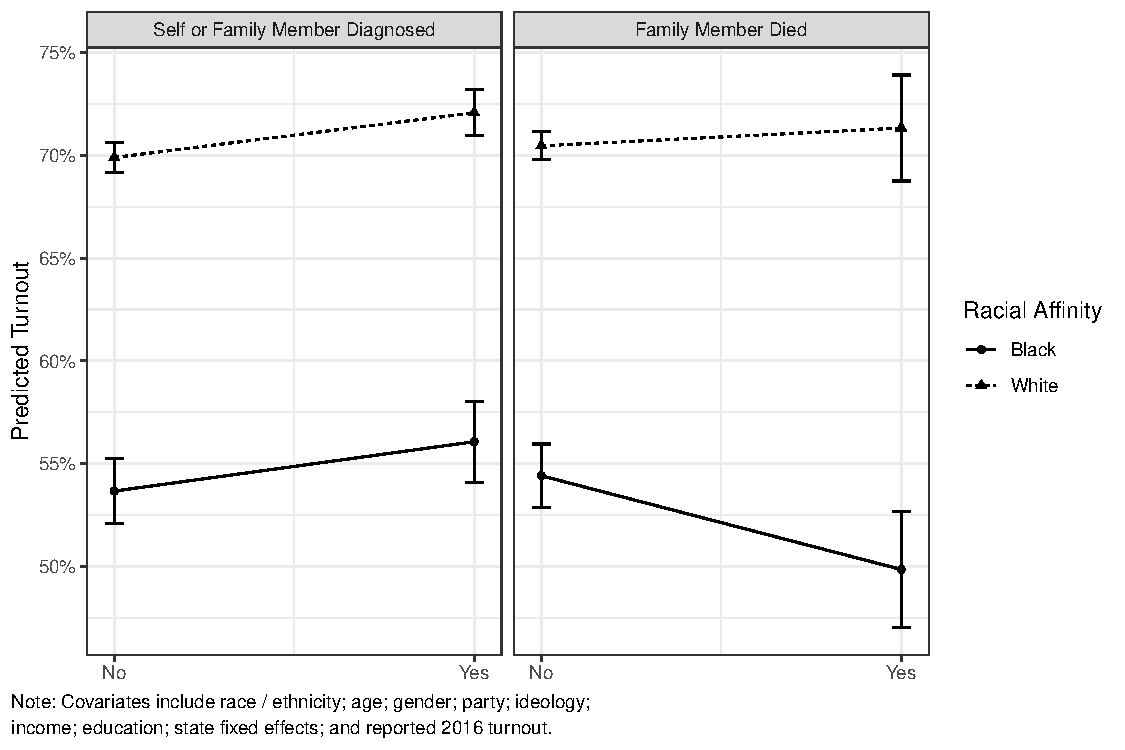
\includegraphics{wa_covid_files/figure-latex/mef1-1} 

}

\caption{\label{fig:mef-ces-1}COVID Contact and Turnout, White and Nonwhite Respondents}\label{fig:mef1}
\end{figure}

Although Figure \ref{fig:mef-ces-1} fails to uncover support for Hypotheses 4, Figure \ref{fig:mef-ces-2} shows that the turnout effects of contact or proximal contact with COVID for nonwhite respondents were highly structured by respondents' resentment scores. The figure plots the relationship between contact and racial resentment for the 25th and 75th percentile of respondents according to their resentment score. The left-hand panel indicates that being diagnosed, or having a family member diagnosed, with COVID was perhaps mobilizing for respondents with high levels of resentment, but that such contact was unassociated with turnout for individuals without such resentment. The right-hand panel, where I test the ``strong'' treatment of having a family member who died from COVID, shows that this contact was associated with much lower turnout for nonwhite voters with low racial resentment toward whites, but had no relationship with turnout for nonwhites with higher scores.

\begin{figure}[H]

{\centering 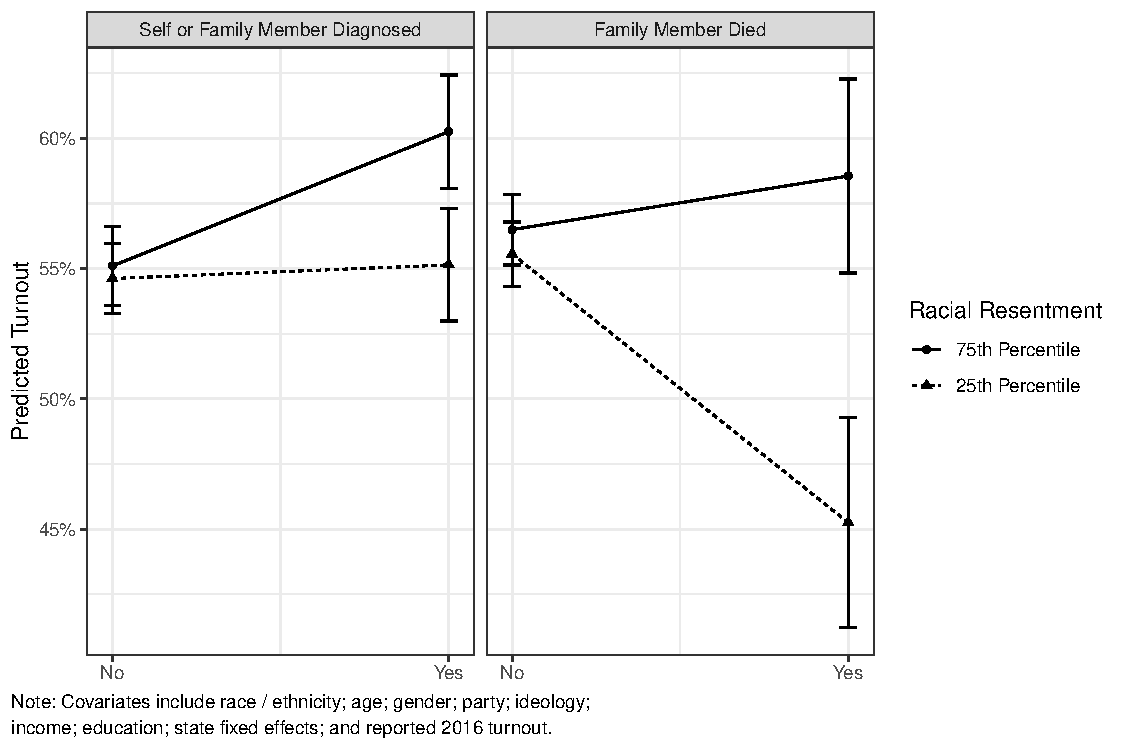
\includegraphics{wa_covid_files/figure-latex/mef2-1} 

}

\caption{\label{fig:mef-ces-2}COVID Contact and Turnout by Racial Affinity, Nonwhite Voters}\label{fig:mef2}
\end{figure}

\hypertarget{blaming-the-government}{%
\subsection*{Blaming the Government}\label{blaming-the-government}}
\addcontentsline{toc}{subsection}{Blaming the Government}

Thanks to the modular structure of the CES in which individual teams ask 1,000 respondents each a series of questions, we can take the results presented in the previous section one step further. In the 2020 CES, the team from the University of Kentucky asked individuals with exposure to Covid who they blamed for the pandemic. Respondents could choose from one of the following options: bad luck; your choices; the economy; the federal government; the state government; the local government; or none of these. Just 537 of their respondents reported contact with Covid, and even fewer were nonwhite. Nevertheless, these data allow us to test whether those with higher levels of resentment were more likely to hold the government responsible for the pandemic. Given that contact was politically mobilizing for individuals with high levels of resentment, this should be the case.

Table \ref{tab:blame} indicates that this was in fact the case. Nonwhite respondents who reported contact with Covid and had high levels of resentment against white racism were considerably more likely to hold the government responsible for the pandemic. Net of other covariates, those at the 25th percentile of this group blamed the government about 21\% of the time; that grew to 37\% for those at the 75th percentile. This provides further corroboration for the results from the previous section: those nonwhite respondents with high levels of resentment were more likely to blame the government for their contact with Covid---and, in turn, voted at considerably higher rates.

{[}insert table{]}

\newpage

\hypertarget{references}{%
\subsection*{References}\label{references}}
\addcontentsline{toc}{subsection}{References}

\hypertarget{refs}{}
\begin{CSLReferences}{1}{0}
\leavevmode\vadjust pre{\hypertarget{ref-Abadie2020}{}}%
Abadie, Alberto, and Jann Spiess. 2020. {``Robust {Post-Matching Inference}.''} \emph{Journal of the American Statistical Association} 0 (0): 1--13. \url{https://doi.org/10.1080/01621459.2020.1840383}.

\leavevmode\vadjust pre{\hypertarget{ref-Blount2020}{}}%
Blount, Linda Goler. 2020. {``Fighting {Injustice} in {Health Care} for {Black Women} and {Diverse Rare Disease Patients}.''} \emph{Ebony}, July.

\leavevmode\vadjust pre{\hypertarget{ref-Blow2020}{}}%
Blow, Charles M. 2020. {``Can {We Call Trump} a {Killer}?''} \emph{The New York Times}, June.

\leavevmode\vadjust pre{\hypertarget{ref-Calia2020}{}}%
Calia, Mike. 2020. {``Full Interview: {President Trump} Discusses Trade, Impeachment, {Boeing} and {Elon Musk} with {CNBC} in {Davos}.''} \emph{CNBC}, January.

\leavevmode\vadjust pre{\hypertarget{ref-Campbell2003a}{}}%
Campbell, Andrea Louise. 2003. {``Participatory {Reactions} to {Policy Threats}: {Senior Citizens} and the {Defense} of {Social Security} and {Medicare}.''} \emph{Political Behavior} 25 (1): 29--49. \url{https://doi.org/10.1023/A:1022900327448}.

\leavevmode\vadjust pre{\hypertarget{ref-cdc2021}{}}%
{``Cases, {Data}, and {Surveillance}.''} 2021. \emph{Centers for Disease Control and Prevention}. https://www.cdc.gov/coronavirus/2019-ncov/covid-data/investigations-discovery/hospitalization-death-by-race-ethnicity.html.

\leavevmode\vadjust pre{\hypertarget{ref-nyt2020}{}}%
{``Covid in the {U}.{S}.: {Latest Map} and {Case Count}.''} 2020. \emph{New York Times}, November.

\leavevmode\vadjust pre{\hypertarget{ref-Davis2021}{}}%
Davis, Darren W., and David C. Wilson. 2021. \emph{Racial {Resentment} in the {Political Mind}}. \emph{Racial Resentment in the Political Mind}. {University of Chicago Press}. \url{https://doi.org/10.7208/chicago/9780226814704}.

\leavevmode\vadjust pre{\hypertarget{ref-Douglas2020}{}}%
Douglas, Jason. 2020. {``As {Coronavirus Surges} in {U}.{S}., {Some Countries Have Just About Halted It}.''} \emph{Wall Street Journal}, July.

\leavevmode\vadjust pre{\hypertarget{ref-Egede2020}{}}%
Egede, Leonard E., and Rebekah J. Walker. 2020. {``Structural {Racism}, {Social Risk Factors}, and {Covid-19} \textemdash{} {A Dangerous Convergence} for {Black Americans}.''} \emph{New England Journal of Medicine} 383 (12): e77. \url{https://doi.org/10.1056/NEJMp2023616}.

\leavevmode\vadjust pre{\hypertarget{ref-Emmenegger2015}{}}%
Emmenegger, Patrick, Paul Marx, and Dominik Schraff. 2015. {``Labour Market Disadvantage, Political Orientations and Voting: How Adverse Labour Market Experiences Translate into Electoral Behaviour.''} \emph{Socio-Economic Review} 13 (2): 189--213. \url{https://doi.org/10.1093/ser/mwv003}.

\leavevmode\vadjust pre{\hypertarget{ref-Fan2004}{}}%
Fan, Jessie X., and Cathleen D. Zick. 2004. {``The {Economic Burden} of {Health Care}, {Funeral}, and {Burial Expenditures} at the {End} of {Life}.''} \emph{Journal of Consumer Affairs} 38 (1): 35--55. \url{https://doi.org/10.1111/j.1745-6606.2004.tb00464.x}.

\leavevmode\vadjust pre{\hypertarget{ref-Fitzpatrick2020}{}}%
Fitzpatrick, Alex. 2020. {``Why the {U}.{S}. {Is Losing} the {War On COVID-19}.''} \emph{Time}, August.

\leavevmode\vadjust pre{\hypertarget{ref-Frum2020}{}}%
Frum, David. 2020. {``This {Is Trump}'s {Plague Now}.''} \emph{The Atlantic}. https://www.theatlantic.com/ideas/archive/2020/06/this-is-trumps-plague-now/613633/.

\leavevmode\vadjust pre{\hypertarget{ref-Garg2020}{}}%
Garg, Shikha, Lindsay Kim, Michael Whitaker, Alissa O'Halloran, Charisse Cummings, Rachel Holstein, Mila Prill, et al. 2020. {``Hospitalization {Rates} and {Characteristics} of {Patients Hospitalized} with {Laboratory-Confirmed Coronavirus Disease} 2019 \textemdash{} {COVID-NET}, 14 {States}, {March} 1\textendash 30, 2020.''} \emph{MMWR. Morbidity and Mortality Weekly Report} 69 (15): 458--64. \url{https://doi.org/10.15585/mmwr.mm6915e3}.

\leavevmode\vadjust pre{\hypertarget{ref-Golden2020}{}}%
Golden, Hallie. 2020. {``Coronavirus: {Washington} State at Center of {US} Outbreak as 18 Cases Confirmed.''} \emph{The Guardian}, March.

\leavevmode\vadjust pre{\hypertarget{ref-Hassell2017}{}}%
Hassell, Hans J. G., and Jaime E. Settle. 2017. {``The {Differential Effects} of {Stress} on {Voter Turnout}.''} \emph{Political Psychology} 38 (3): 533--50. \url{https://doi.org/10.1111/pops.12344}.

\leavevmode\vadjust pre{\hypertarget{ref-Hobbs2014}{}}%
Hobbs, William R., Nicholas A. Christakis, and James H. Fowler. 2014. {``Widowhood {Effects} in {Voter Participation}.''} \emph{American Journal of Political Science} 58 (1): 1--16. \url{https://doi.org/10.1111/ajps.12040}.

\leavevmode\vadjust pre{\hypertarget{ref-HoSang2010}{}}%
HoSang, Daniel. 2010. \emph{Racial Propositions: Ballot {Initiatives} and the Making of Postwar {California}}. American Crossroads 30. {Berkeley}: {University of California Press}.

\leavevmode\vadjust pre{\hypertarget{ref-Imai2016}{}}%
Imai, Kosuke, and Kabir Khanna. 2016. {``Improving {Ecological Inference} by {Predicting Individual Ethnicity} from {Voter Registration Records}.''} \emph{Political Analysis} 24 (2): 263--72. \url{https://doi.org/10.1093/pan/mpw001}.

\leavevmode\vadjust pre{\hypertarget{ref-Imai2020}{}}%
Imai, Kosuke, In Song Kim, and Erik Wang. 2020. {``Matching {Methods} for {Causal Inference} with {Time-Series Cross-Sectional Data}.''} \emph{Working Paper}. \href{https://doi.org/Matching\%20Methods\%20for\%20Causal\%20Inference\%20with\%20Time-Series\%20Cross-Sectional\%20Data}{https://doi.org/Matching Methods for Causal Inference with Time-Series Cross-Sectional Data}.

\leavevmode\vadjust pre{\hypertarget{ref-Johnson-Agbakwu2020}{}}%
Johnson-Agbakwu, Crista E., Nyima S. Ali, Corrina M. Oxford, Shana Wingo, Emily Manin, and Dean V. Coonrod. 2020. {``Racism, {COVID-19}, and {Health Inequity} in the {USA}: A {Call} to {Action}.''} \emph{Journal of Racial and Ethnic Health Disparities}, November, 1--7. \url{https://doi.org/10.1007/s40615-020-00928-y}.

\leavevmode\vadjust pre{\hypertarget{ref-Karaca-Mandic2021}{}}%
Karaca-Mandic, Pinar, Archelle Georgiou, and Soumya Sen. 2021. {``Assessment of {COVID-19 Hospitalizations} by {Race}/{Ethnicity} in 12 {States}.''} \emph{JAMA Internal Medicine} 181 (1): 131--34. \url{https://doi.org/10.1001/jamainternmed.2020.3857}.

\leavevmode\vadjust pre{\hypertarget{ref-Kolata2020}{}}%
Kolata, Gina, and Roni Caryn Rabin. 2020. {``{`{Don}'t {Be Afraid} of {Covid},'} {Trump Says}, {Undermining Public Health Messages}.''} \emph{The New York Times}, October.

\leavevmode\vadjust pre{\hypertarget{ref-Lerman2014}{}}%
Lerman, Amy E., and Vesla M. Weaver. 2014. \emph{Arresting Citizenship: The Democratic Consequences of {American} Crime Control}. Chicago Studies in {American} Politics. {Chicago}: {The University of Chicago Press}.

\leavevmode\vadjust pre{\hypertarget{ref-Lu2020}{}}%
Lu, Denise. 2020. {``The {True Coronavirus Toll} in the {U}.{S}. {Has Already Surpassed} 200,000.''} \emph{The New York Times}, August.

\leavevmode\vadjust pre{\hypertarget{ref-Margalit2019}{}}%
Margalit, Yotam. 2019. {``Political {Responses} to {Economic Shocks}.''} \emph{Annual Review of Political Science} 22 (1): 277--95. \url{https://doi.org/10.1146/annurev-polisci-050517-110713}.

\leavevmode\vadjust pre{\hypertarget{ref-Marx2016}{}}%
Marx, Paul, and Christoph Nguyen. 2016. {``Are the {Unemployed Less Politically Involved}? {A Comparative Study} of {Internal Political Efficacy}.''} \emph{European Sociological Review} 32 (5): 634--48. \url{https://doi.org/10.1093/esr/jcw020}.

\leavevmode\vadjust pre{\hypertarget{ref-McNerthney2020}{}}%
McNerthney, Casey. 2020. {``Coronavirus in {Washington} State: {A} Timeline of the Outbreak Through {March} 2020.''} \emph{KIRO}, April.

\leavevmode\vadjust pre{\hypertarget{ref-Moon2020}{}}%
Moon, Sarah. 2020. {``A Seemingly Healthy Woman's Sudden Death Is Now the First Known {US} Coronavirus-Related Fatality.''} \emph{CNN}, April.

\leavevmode\vadjust pre{\hypertarget{ref-Mystal2020}{}}%
Mystal, Elie. 2020. {``The {Deaths} of 150,000 {Americans Are} on {Trump}'s {Hands},''} August.

\leavevmode\vadjust pre{\hypertarget{ref-Nichols2020a}{}}%
Nichols, Vanessa Cruz, and Ramón Garibaldo Valdéz. 2020. {``How to {Sound} the {Alarms}: {Untangling Racialized Threat} in {Latinx Mobilization}.''} \emph{PS: Political Science \& Politics} 53 (4): 690--96. \url{https://doi.org/10.1017/S1049096520000530}.

\leavevmode\vadjust pre{\hypertarget{ref-Niemi1991}{}}%
Niemi, Richard G., Stephen C. Craig, and Franco Mattei. 1991. {``Measuring {Internal Political Efficacy} in the 1988 {National Election Study}.''} \emph{The American Political Science Review} 85 (4): 1407--13. \url{https://doi.org/10.2307/1963953}.

\leavevmode\vadjust pre{\hypertarget{ref-Pacheco2015}{}}%
Pacheco, Julianna, and Jason Fletcher. 2015. {``Incorporating {Health} into {Studies} of {Political Behavior}: {Evidence} for {Turnout} and {Partisanship}.''} \emph{Political Research Quarterly} 68 (1): 104--16. \url{https://doi.org/10.1177/1065912914563548}.

\leavevmode\vadjust pre{\hypertarget{ref-Perez2015}{}}%
Pérez, Efrén O. 2015. {``Xenophobic {Rhetoric} and {Its Political Effects} on {Immigrants} and {Their Co-Ethnics}.''} \emph{American Journal of Political Science} 59 (3): 549--64.

\leavevmode\vadjust pre{\hypertarget{ref-Piven1979}{}}%
Piven, Frances Fox, and Richard A. Cloward. 1979. \emph{Poor People's Movements: Why They Succeed, How They Fail}. {New York}: {Vintage books}.

\leavevmode\vadjust pre{\hypertarget{ref-whitehouse2020}{}}%
{``Remarks by {President Trump} at a {USMCA Celebration} with {American Workers}.''} 2020. \emph{The White House}. https://www.whitehouse.gov/briefings-statements/remarks-president-trump-usmca-celebration-american-workers-warren-mi/.

\leavevmode\vadjust pre{\hypertarget{ref-Robinson2020}{}}%
Robinson, Ishena. 2020. {``{CDC}'s {New Numbers Show Black Americans} and {Other People} of {Color Dying} at {Higher Rates From COVID-19 Than It Previously Reported}.''} \emph{The Root}, December.

\leavevmode\vadjust pre{\hypertarget{ref-Rosenstone1982}{}}%
Rosenstone, Steven J. 1982. {``Economic {Adversity} and {Voter Turnout}.''} \emph{American Journal of Political Science} 26 (1): 25--46. \url{https://doi.org/10.2307/2110837}.

\leavevmode\vadjust pre{\hypertarget{ref-Rudolph2000}{}}%
Rudolph, Thomas J., Amy Gangl, and Dan Stevens. 2000. {``The {Effects} of {Efficacy} and {Emotions} on {Campaign Involvement}.''} \emph{The Journal of Politics} 62 (4): 1189--97. \url{https://doi.org/10.1111/0022-3816.00053}.

\leavevmode\vadjust pre{\hypertarget{ref-Saletan2020}{}}%
Saletan, William. 2020. {``How {Trump Killed Tens} of {Thousands} of {Americans}.''} \emph{Slate Magazine}. https://slate.com/news-and-politics/2020/08/trump-coronavirus-deaths-timeline.html.

\leavevmode\vadjust pre{\hypertarget{ref-Sandell2005}{}}%
Sandell, Julianna, and Eric Plutzer. 2005. {``Families, Divorce and Voter Turnout in the {US}.''} \emph{Political Behavior} 27 (2): 133--62. \url{https://doi.org/10.1007/s11109-005-3341-9}.

\leavevmode\vadjust pre{\hypertarget{ref-Schlozman1979}{}}%
Schlozman, Kay Kehman, and Sidney Verba. 1979. \emph{Injury to {Insult}: {Unemployment}, {Class}, and {Political Response}}. {Harvard University Press}.

\leavevmode\vadjust pre{\hypertarget{ref-Sciarini2016}{}}%
Sciarini, Pascal, and Andreas C. Goldberg. 2016. {``Turnout {Bias} in {Postelection Surveys}: {Political Involvement}, {Survey Participation}, and {Vote Overreporting}.''} \emph{Journal of Survey Statistics and Methodology} 4 (1): 110--37. \url{https://doi.org/10.1093/jssam/smv039}.

\leavevmode\vadjust pre{\hypertarget{ref-Sekhon2011}{}}%
Sekhon, Jasjeet S. 2011. {``Multivariate and {Propensity Score Matching Software} with {Automated Balance Optimization}: {The Matching} Package for {R}.''} \emph{Journal of Statistical Software} 42 (7): 1--52. \url{https://doi.org/10.18637/jss.v042.i07}.

\leavevmode\vadjust pre{\hypertarget{ref-Shear2020}{}}%
Shear, Michael D., Noah Weiland, Eric Lipton, Maggie Haberman, and David E. Sanger. 2020. {``Inside {Trump}'s {Failure}: {The Rush} to {Abandon Leadership Role} on the {Virus}.''} \emph{The New York Times}, July.

\leavevmode\vadjust pre{\hypertarget{ref-Tarrow1998}{}}%
Tarrow, Sidney G. 1998. \emph{Power in Movement: Social Movements and Contentious Politics}. 2nd ed. Cambridge Studies in Comparative Politics. {Cambridge {[}England{]} ; New York}: {Cambridge University Press}.

\leavevmode\vadjust pre{\hypertarget{ref-Towler2018}{}}%
Towler, Christopher C., and Christopher S. Parker. 2018. {``Between {Anger} and {Engagement}: {Donald Trump} and {Black America}.''} \emph{Journal of Race, Ethnicity, and Politics} 3 (1): 219--53. \url{https://doi.org/10.1017/rep.2017.38}.

\leavevmode\vadjust pre{\hypertarget{ref-Valenzuela2016}{}}%
Valenzuela, Ali A., and Melissa R. Michelson. 2016. {``Turnout, {Status}, and {Identity}: {Mobilizing Latinos} to {Vote} with {Group Appeals}.''} \emph{American Political Science Review} 110 (4): 615--30. \url{https://doi.org/10.1017/S000305541600040X}.

\leavevmode\vadjust pre{\hypertarget{ref-Wan2020}{}}%
Wan, William. 2020. {``{WHO} Declares a Pandemic of Coronavirus Disease Covid-19.''} \emph{Washington Post}, March.

\leavevmode\vadjust pre{\hypertarget{ref-Weaver2010}{}}%
Weaver, Vesla M., and Amy E. Lerman. 2010. {``Political {Consequences} of the {Carceral State}.''} \emph{American Political Science Review} 104 (4): 817--33. \url{https://doi.org/10.1017/S0003055410000456}.

\leavevmode\vadjust pre{\hypertarget{ref-White2016}{}}%
White, Ariel. 2016. {``When {Threat Mobilizes}: {Immigration Enforcement} and {Latino Voter Turnout}.''} \emph{Political Behavior} 38 (2): 355--82. \url{https://doi.org/10.1007/s11109-015-9317-5}.

\leavevmode\vadjust pre{\hypertarget{ref-Wyatt1999}{}}%
Wyatt, Gwen K., Laurie Friedman, Charles W. Given, and Barbara A. Given. 1999. {``A {Profile} of {Bereaved Caregivers} Following {Provision} of {Terminal Care}.''} \emph{Journal of Palliative Care} 15 (1): 13--25. \url{https://doi.org/10.1177/082585979901500103}.

\leavevmode\vadjust pre{\hypertarget{ref-Zepeda-Millan2017}{}}%
Zepeda-Millán, Chris. 2017. \emph{Latino Mass Mobilization: Immigration, Racialization, and Activism}. First published 2017. {Cambridge, United Kingdom New York Melbourne}: {Cambridge University Press}.

\end{CSLReferences}

\end{document}
